\documentclass{article}
\usepackage{graphicx} 
\usepackage{pgf-pie}
\usepackage[colorlinks=true, urlcolor=blue]{hyperref}

\title{Course logistics}
\date{}

\begin{document}

\maketitle


\section{DSA (CS213 and CS293)}

    \subsection{Course Website}

        \subsubsection{CS213}
        Lecture Slides : \\\url{https://robin.bodhi.cse.iitb.ac.in/courseware/course/195/content/multimedia/coursecontent/}

        \subsubsection{CS293}
        Labs : \\
        \url{https://robin.bodhi.cse.iitb.ac.in/courseware/course/195/content/labs}
        \\\\
        Lab seat mapping : \\\url{https://bit.ly/A26-DSA-Mapping}
    \subsection{Quizzes}

        \subsubsection{CS213}
        Theory Quiz 1 : Thusday, 27th August 2026 (Lecture Slot)
        \subsubsection{CS293}
        Lab Quiz 1 : Tuesday, 25th August 2026 (Lab Slot)
    \subsection{Grade Distribution}

        \subsubsection{CS213 (Theory)}
        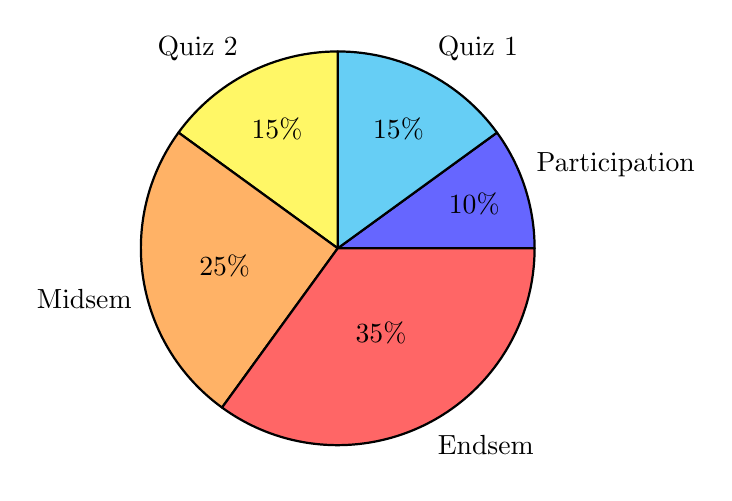
\begin{tikzpicture}
        \pie[radius=2.5]{10/Participation, 15/Quiz 1, 15/Quiz 2, 25/Midsem, 35/Endsem}
        \end{tikzpicture}

        \subsubsection{CS293 (Lab)}
        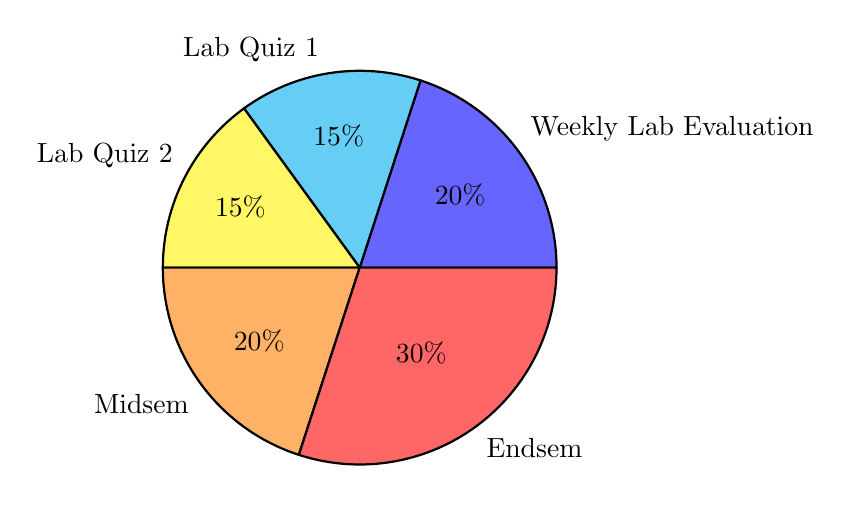
\begin{tikzpicture}
        \pie[radius=2.5]{20/Weekly Lab Evaluation, 15/Lab Quiz 1, 15/Lab Quiz 2, 20/Midsem, 30/Endsem}
        \end{tikzpicture}

    

\pagebreak


\section{DLDCA (CS230 and CS231)}

    \subsection{Course Websites}

        \subsubsection{CS230}
        Course Information + Lecture Slides : \\\url{https://cs230-iitb.github.io/autumn-2026/}\\\\
        Discussion Portal (Piazza) : \\\url{https://piazza.com/class/ms1a6g1fg1luv}

        \subsubsection{CS231}
        Labs : \\
        \url{https://github.com/CS231-DLDCA-Lab/CS231-2026}
        \\\\
        Lab seat mapping : \\\url{https://docs.google.com/spreadsheets/d/1tayAATniMwQ7fh3_62BuHnNRad7Ltvios91gzEG3gZ0/edit?usp=sharing}

        \subsection{Quizzes}

        \subsubsection{CS230}
        Theory Quiz 1 : September 1st Week

    \subsection{Grade Distribution}

        \subsubsection{CS230 (Theory)}
        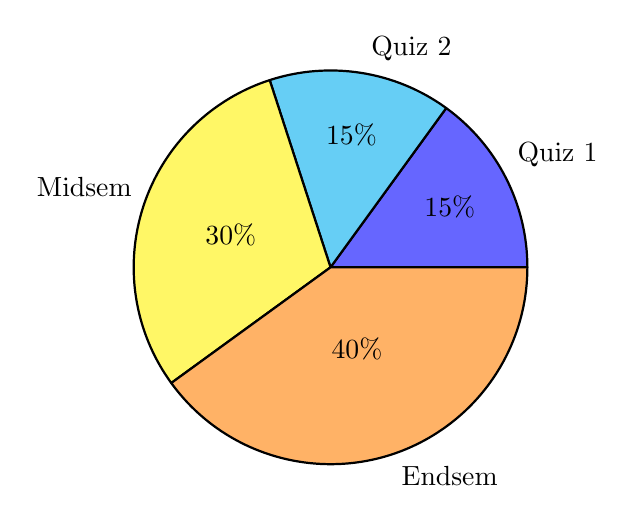
\begin{tikzpicture}
        \pie[radius=2.5]{15/Quiz 1, 15/Quiz 2, 30/Midsem, 40/Endsem}
        \end{tikzpicture}

        \subsubsection{CS231 (Lab)}
        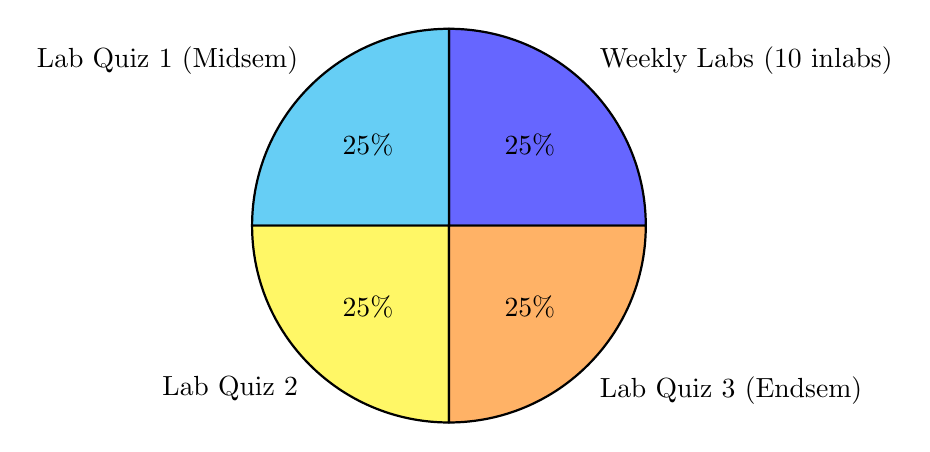
\begin{tikzpicture}
        \pie[radius=2.5]{25/Weekly Labs (10 inlabs), 25/Lab Quiz 1 (Midsem), 25/Lab Quiz 2, 25/Lab Quiz 3 (Endsem)}
        \end{tikzpicture}

\pagebreak


\section{Logic (CS228)}

    \subsection{Course websites}
    Course Content + Lecture slides: \\\url{https://www.cse.iitb.ac.in/~akshayss/courses/cs228-2026/cs228-2026.html}
    \\\\
    Class discussion (Piazza) : \\\url{https://piazza.com/class/ms4gwv81ixb3l0}

    \section{Quizzes}

        \subsection{CS230}
        Quiz 1 : 28th August 2026
    \subsection{Grade Distribution}
    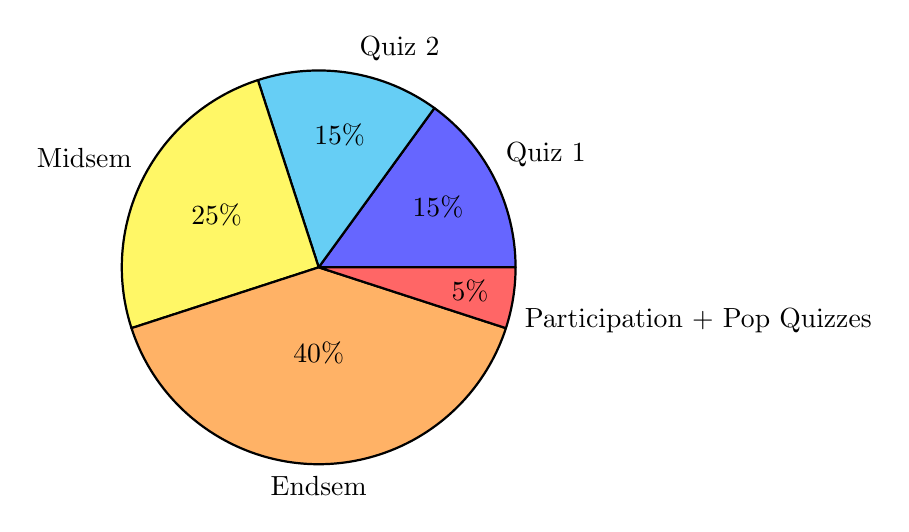
\begin{tikzpicture}
        \pie[radius=2.5]{15/Quiz 1, 15/Quiz 2, 25/Midsem, 40/Endsem, 5/Participation + Pop Quizzes}
    \end{tikzpicture}

\pagebreak


\section{DAI (CS215)}

    \subsection{Course websites}
    Class discussion (Piazza) : \\\url{https://piazza.com/class/ms1ll7021ih5yc}
    \\\\Lecture Slides (Piazza) : \\\url{https://piazza.com/class/ms1ll7021ih5yc#folder=lecturenotes}

    \section{Grade Distribution}
Note that these are approximate values (Midsem : 25-30\%, Endsem : 64-67\%, Attendance + Participation : 5-7\%).\\\\
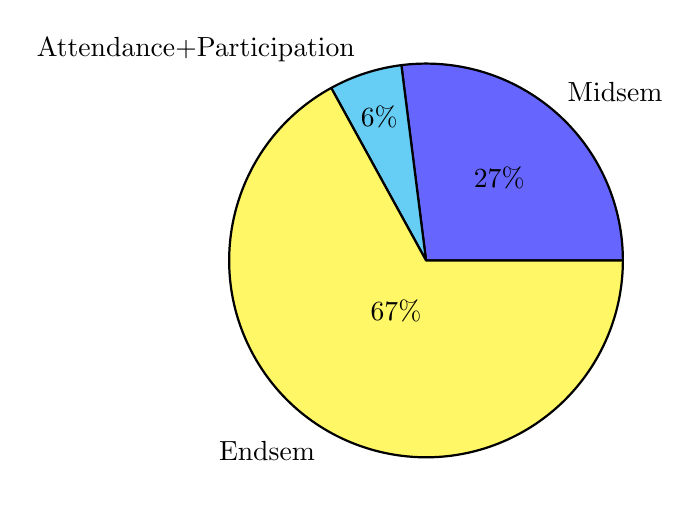
\begin{tikzpicture}
    \pie[radius=2.5]{
        27/Midsem,
        6/Attendance+Participation,
        67/Endsem
    }
\end{tikzpicture}


\end{document}
